\documentclass[11pt,twocolumn]{article}

\usepackage[a4paper,margin=0.6in]{geometry}
\usepackage{amsmath,amssymb,graphicx}
\usepackage{booktabs}
\usepackage{hyperref}
\usepackage{float}
\usepackage{caption}
\usepackage{xcolor}
\usepackage{listings}

\graphicspath{{figures/}{./}}

\lstset{basicstyle=\ttfamily\small,backgroundcolor=\color{gray!8},frame=single,breaklines=true,columns=fullflexible}

% Visible marker for the parts that wait for results (remove before submission)
\newcommand{\todo}[1]{\par\noindent\fcolorbox{red}{yellow!20}{\parbox{0.95\linewidth}{\small\textbf{TODO:} #1}}\par}

\newcommand{\Mpch}{\,h^{-1}\mathrm{Mpc}}

\title{Environment-dependent galaxy clustering from ASTRA tessellations:\\
a comparison with density-split clustering on DESI-like mocks}
\author{Hugo Nguyen}
\date{}

\begin{document}

\maketitle

\begin{abstract}
The large-scale distribution of galaxies contains cosmological information that is only partially captured by two-point statistics. Density-split clustering, which measures the clustering of regions ranked by their smoothed local density, has been shown to recover a significant part of this non-Gaussian information. In this work we study an alternative definition of the local environment based on ASTRA, a parameter-free estimator built on the Delaunay tessellation of the galaxies together with a uniform random catalogue. Using AbacusSummit halo occupation distribution (HOD) mocks reproducing the clustering of DESI luminous red galaxies at $z=0.5$, we measure the monopole and quadrupole of the auto- and cross-correlation functions of ASTRA environment quartiles, and compare them with the standard density-split statistics measured on exactly the same random points. Covariance matrices are estimated from 192 subvolumes of $(500\Mpch)^3$ of the fiducial simulation, and derivatives with respect to $\omega_b$, $\omega_{\rm cdm}$, $n_s$ and $\sigma_8$ from paired differences of HOD-matched simulations of the AbacusSummit derivative grid. We use these products to compare the Fisher information of ASTRA split, density split and the galaxy two-point correlation function.
\todo{Final sentence with the main quantitative result (gain of ASTRA split vs 2PCF and vs density split) once the Fisher forecasts are final.}
\end{abstract}

% =====================================================================
\section{Introduction}
% =====================================================================

The large-scale distribution of galaxies is one of the most powerful probes of modern cosmology. Measurements of galaxy clustering constrain the expansion history of the Universe, the growth rate of structure, the matter density, and the properties of dark energy and neutrinos. Current spectroscopic surveys such as DESI provide galaxy samples of unprecedented volume and statistical precision, creating new opportunities to test the standard cosmological model and its extensions.

In most analyses, cosmological information is compressed into two-point statistics, namely the correlation function in configuration space or the power spectrum in Fourier space. These observables are optimal for Gaussian random fields and remain extremely successful on large scales. However, the late-time matter distribution becomes strongly non-Gaussian through non-linear gravitational evolution, halo formation and redshift-space distortions (RSD). As a result, part of the available cosmological information is not captured by two-point summaries alone.

This limitation has motivated a wide range of complementary statistics: higher-order correlation functions, marked statistics, counts-in-cells, void statistics, and methods based on an explicit segmentation of the cosmic web into nodes, filaments, walls and underdense regions. By conditioning clustering measurements on environment, these methods access information on the local geometry of structure formation and can break parameter degeneracies that remain in standard analyses.

Among them, density-split clustering \cite{Paillas2023, Paillas2024} has shown strong promise: random query points are ranked by the smoothed galaxy density around them, split into quantiles, and the auto-correlation of each quantile and its cross-correlation with the galaxies are measured. Combined with a simulation-based emulator \cite{CuestaLazaro2024}, these statistics improve the constraints on $\Lambda$CDM parameters by factors of several with respect to the two-point function.

In this work we investigate an alternative environment estimator based on the ASTRA algorithm, which classifies points of the cosmic web from the Delaunay tessellation of the galaxies together with a uniform random catalogue \cite{ASTRA}. Unlike density split, ASTRA does not rely on a smoothing scale: the environment of a point is defined by its nearest neighbours in the tessellation, i.e.\ by an adaptive, local scale. Our goal is to determine whether ASTRA-defined environment quartiles carry cosmological information beyond the galaxy two-point correlation function, and how they compare to density split when both are measured on the same mocks, with the same random points and the same clustering estimators.

The paper is organised as follows. Section~\ref{sec:sims} presents the simulations, Section~\ref{sec:env} the two environment estimators and their comparison, Section~\ref{sec:clustering} the clustering measurements, Section~\ref{sec:fisher} the covariance, derivatives and Fisher forecasts, and Section~\ref{sec:robustness} the robustness tests. We discuss limitations and perspectives, in particular the extension to an emulator-based inference, in Section~\ref{sec:discussion}.

% =====================================================================
\section{Simulations and mock catalogues}
\label{sec:sims}
% =====================================================================

We use the HOD galaxy catalogues built for the DESI emulator programme on top of the AbacusSummit $N$-body suite \cite{Maksimova2021}. Each simulation evolves $6912^3$ particles in a periodic box of $2\,h^{-1}{\rm Gpc}$; we use the $z=0.5$ snapshot. Halos are populated with galaxies with the AbacusHOD model \cite{Yuan2022} for luminous red galaxies (LRG), whose 12 parameters (central and satellite occupation, velocity bias, environment-based assembly bias) are sampled in the prior of \cite{Yuan2023}. Every catalogue contains $4\times10^6$ galaxies, i.e.\ $\bar n = 5\times10^{-4}\,h^3{\rm Mpc}^{-3}$.

The catalogues are stored as \texttt{c\{cosmo\}\_ph000/seed0/hod\{NNN\}.fits}. Two properties of this suite drive our methodology:
\begin{itemize}
\item \textbf{One phase per cosmology.} All cosmologies share the initial conditions \texttt{ph000}; there is a single HOD seed.
\item \textbf{One HOD draw per file.} The 500 files \texttt{hod000}--\texttt{hod499} of a cosmology have \emph{different} HOD parameters (a Latin hypercube for emulator training), and the parameters behind a given index differ from one cosmology to another.
\end{itemize}
Consequently, different HOD files cannot be used as independent realisations of the same model. The scatter between HOD draws reaches $\sim55\%$ of the amplitude of the density-split monopoles, against $\sim1\%$ for the cosmological response we want to measure. We therefore estimate the covariance from subvolumes of a single catalogue, and derivatives from HOD-matched pairs (Section~\ref{sec:fisher}).

\paragraph{Cosmologies.} Besides the fiducial Planck 2018 $\Lambda$CDM cosmology (\texttt{c000}), we use the AbacusSummit linear derivative grid (Table~\ref{tab:cosmo}). Each pair varies one parameter around the fiducial, with $h$ and $A_s$ adjusted to keep the angular size of the sound horizon $\theta_*$ and, for \texttt{c100}--\texttt{c105}, $\sigma_8$ fixed. Derivatives with respect to $\omega_b$, $\omega_{\rm cdm}$ and $n_s$ are therefore taken at fixed $\sigma_8$.

\begin{table}[h]
\centering\small
\begin{tabular}{lccc}
\toprule
Parameter & fiducial & $+$ / $-$ & step $\theta_+-\theta_-$ \\
\midrule
$\omega_b$ & 0.02237 & c100 / c101 & 0.00089 \\
$\omega_{\rm cdm}$ & 0.1200 & c102 / c103 & 0.0079 \\
$n_s$ & 0.9649 & c104 / c105 & 0.0200 \\
$\sigma_8$ & 0.808 & c112 / c113 & 0.0320 \\
\bottomrule
\end{tabular}
\caption{AbacusSummit cosmologies used for the derivatives.}
\label{tab:cosmo}
\end{table}

\paragraph{Positions.} We place the line of sight along one axis of the box ($z$ by default, $x$ and $y$ for the covariance). Redshift-space positions are \texttt{X\_PERP}, \texttt{Y\_PERP}, \texttt{Z\_RSD}; real-space positions use \texttt{Z\_PERP}. These columns already include the Alcock--Paczynski rescaling of the fiducial cosmology ($q_\perp$, $q_\parallel$, stored in the headers), so the box is $2000/q_\perp$ across and $2000/q_\parallel$ along the line of sight.

% =====================================================================
\section{Environment estimators}
\label{sec:env}
% =====================================================================

Both estimators are evaluated on the \emph{full periodic box}, and on the same set of $N_r = N_g = 4\times10^6$ uniform random points (fixed seed, drawn in the unit cube and rescaled to the box, so that the random points are identical in all cosmologies up to the AP rescaling).

\subsection{ASTRA split}

The galaxies and random points are joined into a single catalogue and Delaunay-triangulated. For every point (galaxy or random) we count the numbers $N_{\rm data}$ and $N_{\rm rand}$ of galaxies and randoms among its Delaunay neighbours and define
\begin{equation}
r = \frac{N_{\rm data}-N_{\rm rand}}{N_{\rm data}+N_{\rm rand}} \in [-1,1].
\label{eq:astra_r}
\end{equation}
A point surrounded by galaxies ($r\to1$) lies in a dense region, a point surrounded by randoms ($r\to-1$) in an underdense one. In the original ASTRA classification, fixed thresholds on $r$ define voids, sheets, filaments and knots; here we only use $r$ as a continuous environment variable.

The triangulation is computed independently in each subvolume (Section~\ref{sec:clustering}) on a region padded by $30\Mpch$ on each side, with periodic wrapping across the faces of the simulation box, and $r$ is kept only for the points inside the subvolume. This removes the edge effects of a non-periodic triangulation (missing neighbours, elongated boundary simplices). The mean inter-point separation of the joint catalogue is $\simeq 10\Mpch$, so that the padding contains several layers of neighbours; we verify the convergence in Section~\ref{sec:robustness}.

\subsection{Density split}

As a reference we use the standard density split \cite{Paillas2023}. The galaxies are assigned to a periodic mesh of $5\Mpch$ cells with a cloud-in-cell scheme, the overdensity field is smoothed with a Gaussian kernel of radius $R_s = 10\Mpch$ by FFT, and the smoothed density contrast $\delta_R$ is read (CIC) at the position of every galaxy and random point.

\subsection{Environment quartiles}

For each method, each subvolume and each population, points are ranked by their environment value ($r$ or $\delta_R$) and split into four quartiles of exactly equal size, Q1 (most underdense) to Q4 (most overdense). Because $r$ is a ratio of small integers, many points share the same value; ties are broken at random. We consider two populations:
\begin{itemize}
\item \textbf{random quartiles}: the random points, ranked by their environment. They play the role of the query points of density split, and sample the environments by volume;
\item \textbf{galaxy quartiles}: the galaxies, ranked by their own environment. They sample the environments by mass.
\end{itemize}
Galaxies and randoms are ranked separately, so that the quartile thresholds of one population do not depend on the other.

\subsection{Comparison of the two classifications}

Figure~\ref{fig:env} compares the two estimators on the fiducial catalogue. They are strongly but not perfectly correlated: the Spearman rank correlation between $r$ and $\delta_R$ is $\rho = 0.719\pm0.005$ for random points and $0.713\pm0.005$ for galaxies (scatter over subvolumes). The extreme quartiles are the most consistent: 63\% of the ASTRA Q1 (Q4) random points are also in the density-split Q1 (Q4), whereas the intermediate quartiles are largely mixed, and less than 2\% of the points move between the two extremes. ASTRA therefore identifies the same large-scale structures as density split, but redistributes a large fraction of the points, as expected from an estimator based on an adaptive (nearest-neighbour) rather than a fixed smoothing scale.

\begin{figure*}[t]
\centering
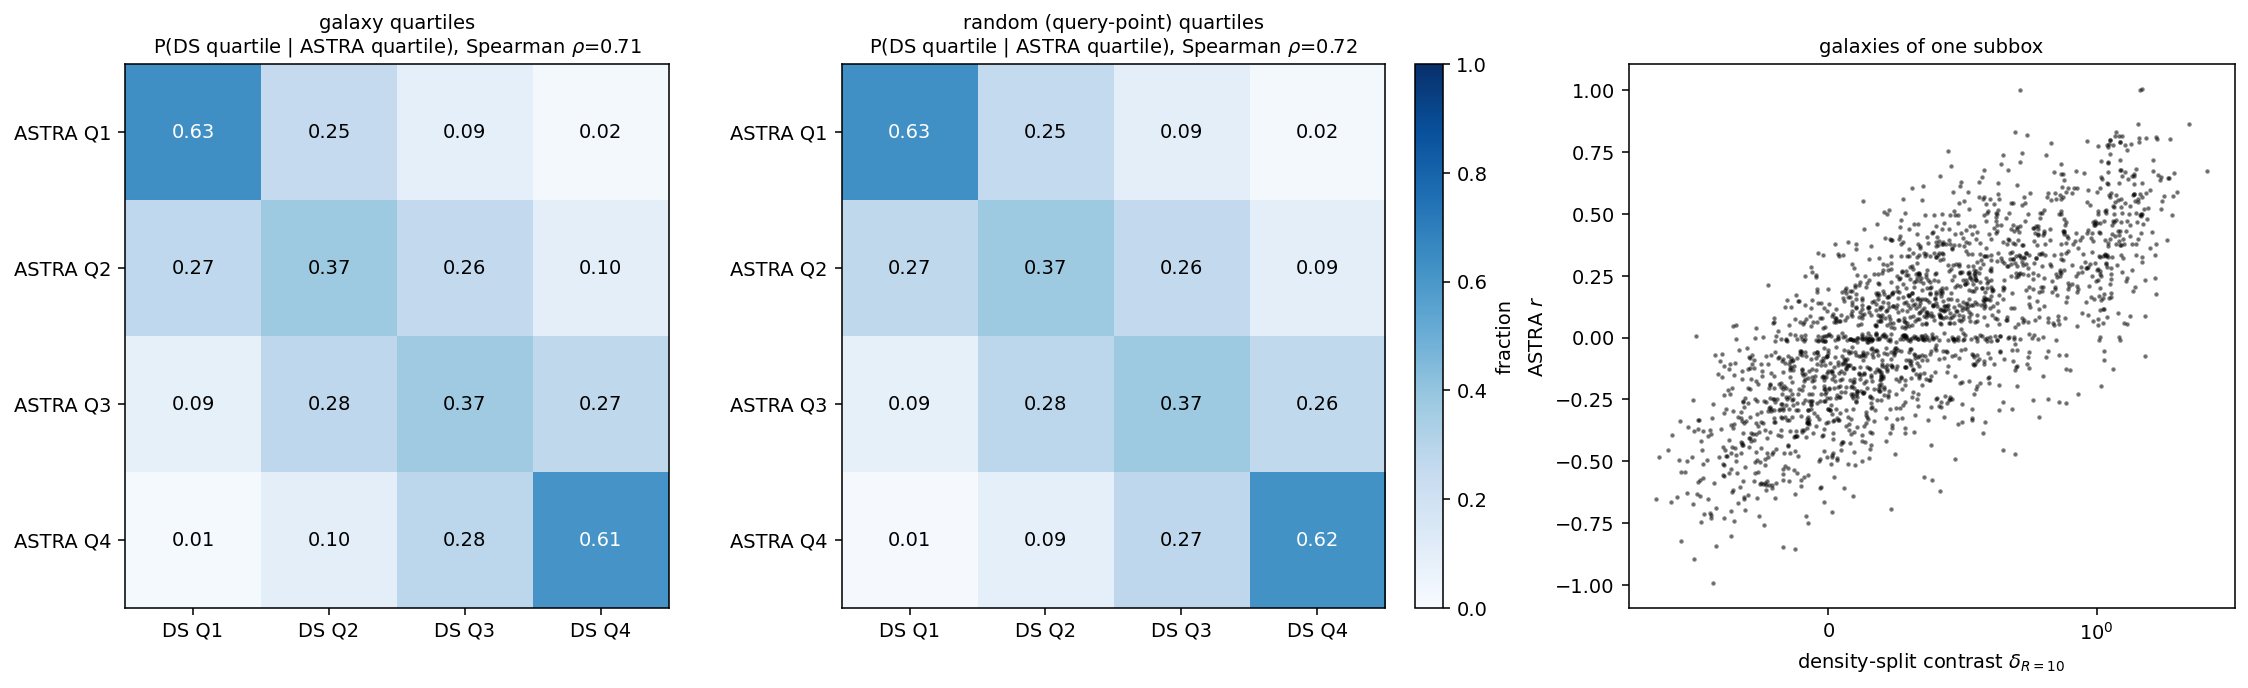
\includegraphics[width=0.95\textwidth]{v2_environment.png}
\caption{Comparison of the ASTRA and density-split environments on the fiducial catalogue (\texttt{c000}, \texttt{hod239}, line of sight $z$). Left and middle: probability that a point of a given ASTRA quartile falls in each density-split quartile, for galaxies and for random points (average over the 64 subvolumes). Right: ASTRA $r$ against the smoothed density contrast $\delta_{R=10}$ for a random sample of galaxies (small vertical jitter added to the discrete $r$ values).}
\label{fig:env}
\end{figure*}

% =====================================================================
\section{Clustering measurements}
\label{sec:clustering}
% =====================================================================

\subsection{Subvolumes and estimator}

Each $2\,h^{-1}{\rm Gpc}$ box is divided into $4^3=64$ non-overlapping cubic subvolumes of $500\Mpch$ (about $62\,500$ galaxies each). Each subvolume is treated as an independent survey with open boundaries: correlation functions are measured with the Landy--Szalay estimator \cite{LandySzalay1993},
\begin{equation}
\xi(s,\mu) = \frac{D_1D_2 - D_1R - RD_2 + RR}{RR},
\end{equation}
using a uniform catalogue of $5\times$ the number of galaxies to describe the geometry (the same for all subvolumes, so that $RR$ is computed once). Pair counts are computed with \texttt{pycorr}/\texttt{Corrfunc} \cite{Sinha2020} in 30 bins of $5\Mpch$ in $s\in[0,150]\Mpch$ and 120 bins in $\mu\in[-1,1]$, with $\mu$ defined with respect to the fixed line of sight, and projected on the Legendre multipoles $\ell=0,2,4$.

\subsection{Statistics}

For each method $m\in\{$ASTRA, DS$\}$, population $p\in\{$random, galaxy$\}$ and quartile Q$_i$ we measure
\begin{itemize}
\item the quartile--galaxy cross-correlation $\xi^{\rm QG}_{i,\ell}(s)$, between the points of Q$_i$ and all galaxies;
\item the quartile auto-correlation $\xi^{\rm QQ}_{i,\ell}(s)$;
\end{itemize}
together with the galaxy two-point correlation function $\xi^{\rm GG}_\ell(s)$ (2PCF). For random quartiles, $\xi^{\rm QG}$ is the analogue of the density-split cross-correlation function and $\xi^{\rm QQ}$ of the density-split auto-correlation function \cite{Paillas2023}.

\subsection{Results on the fiducial cosmology}

Figure~\ref{fig:multipoles_rand} shows the multipoles of the random-quartile statistics for both methods, and Figure~\ref{fig:multipoles_gal} those of the galaxy quartiles.

The two methods produce qualitatively identical signals. The Q1--galaxy cross-correlation is negative at small separations, the profile of galaxies around underdense regions, and the Q4--galaxy cross-correlation is positive and above the galaxy 2PCF, the profile around overdense regions. Both auto-correlations of the extreme quartiles are strongly enhanced with respect to the galaxy 2PCF. The quadrupoles have opposite signs for Q1 and Q4: around underdense regions, peculiar velocities point outwards and stretch the void profile along the line of sight, while around overdense regions infall compresses it. The intermediate quartiles Q2--Q3 carry a weak signal, close to the mean field.

The ASTRA signals are systematically weaker than the density-split ones, by a factor $\sim1.6$ at the peak of the Q1 and Q4 cross-correlations ($s^2\xi_0 \simeq -90$ and $+90\,h^{-2}{\rm Mpc}^2$, against $-145$ and $+145$ for density split). This is consistent with the partial mixing of the quartiles (Figure~\ref{fig:env}): the ASTRA estimator is noisier at fixed point, since it relies on $\sim15$ neighbours only, which dilutes the contrast between environments. The relevant question is however not the amplitude of the signal but its information content relative to its noise, which we address with the Fisher analysis.

\begin{figure*}[t]
\centering
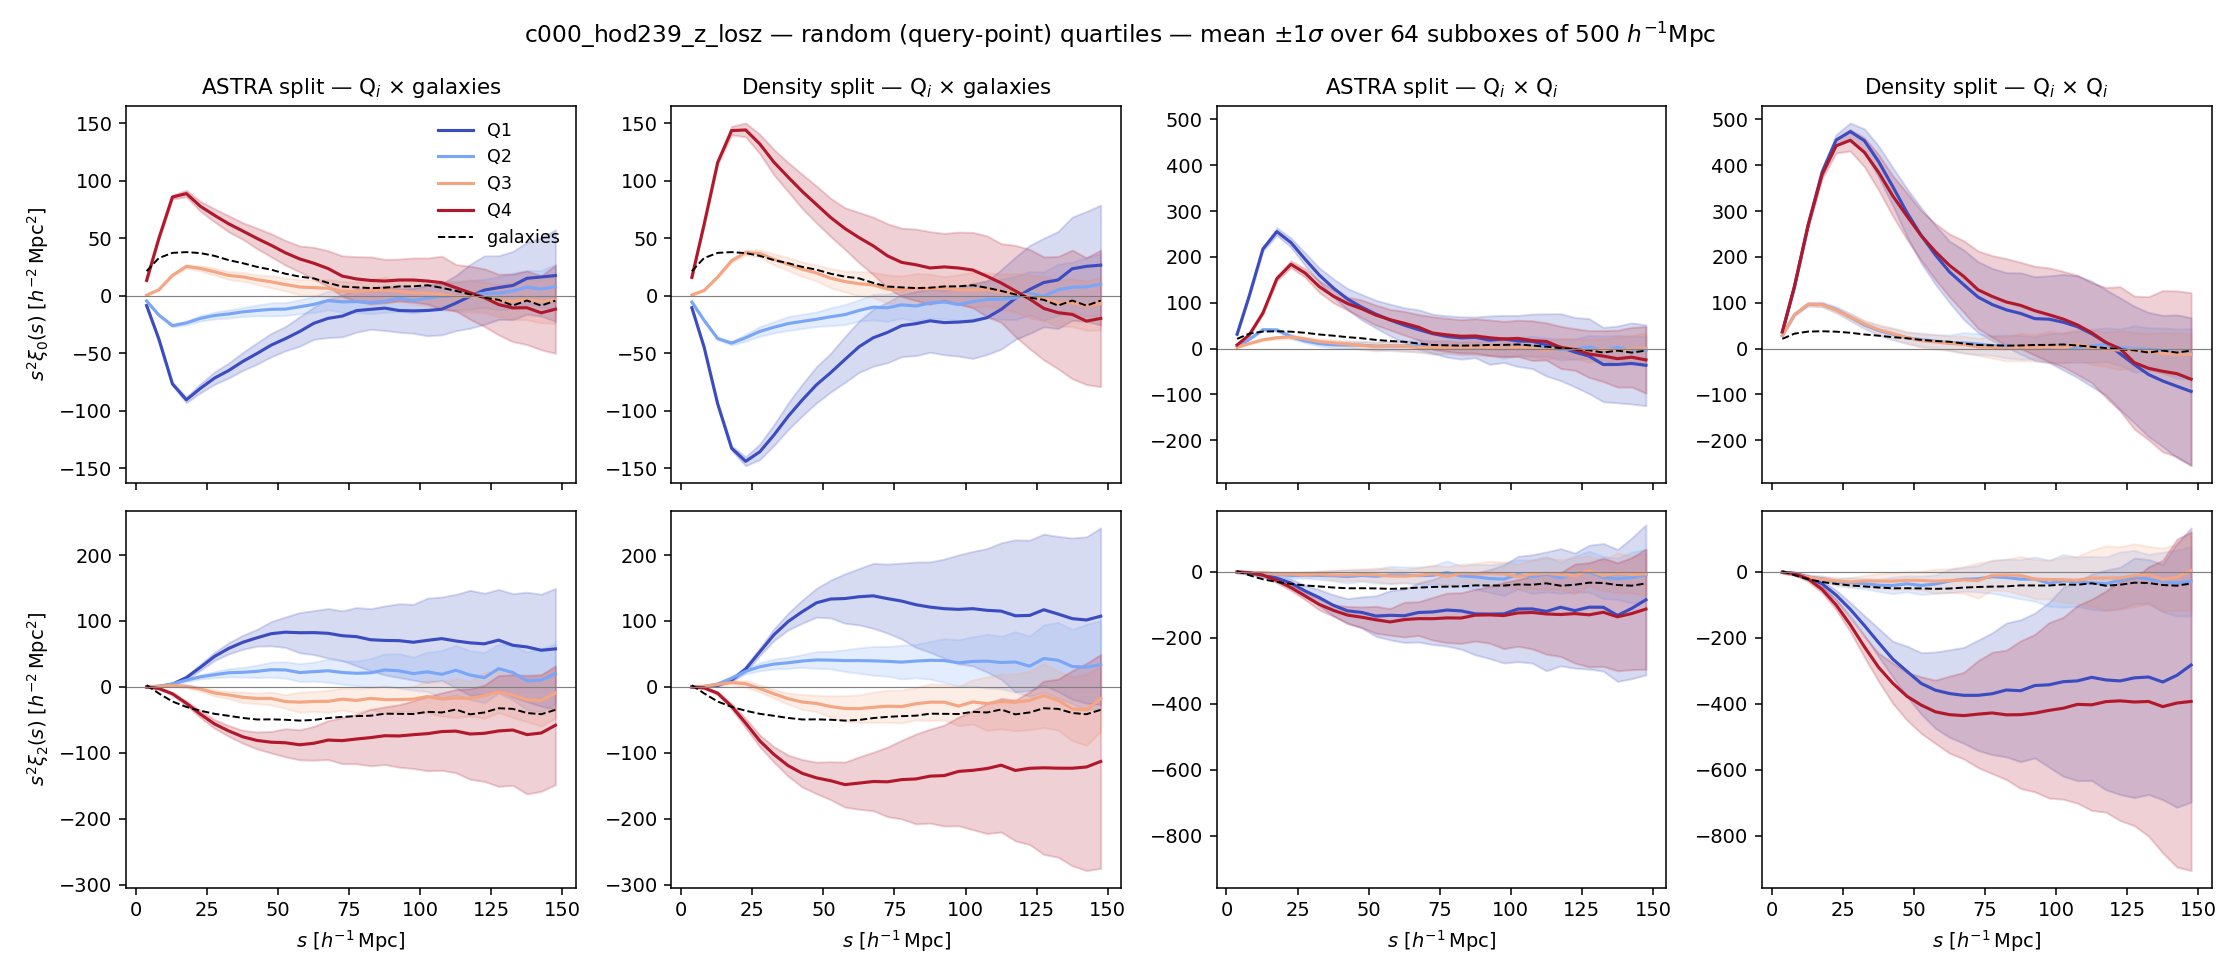
\includegraphics[width=\textwidth]{v2_multipoles_rand.png}
\caption{Monopole (top) and quadrupole (bottom) of the random-quartile statistics on the fiducial catalogue, for ASTRA split and density split: quartile--galaxy cross-correlations (two left columns) and quartile auto-correlations (two right columns), from Q1 (most underdense, blue) to Q4 (most overdense, red). The dashed line is the galaxy 2PCF. Lines and bands are the mean and $1\sigma$ scatter over the 64 subvolumes of $(500\Mpch)^3$; panels of the same statistic share the same scale.}
\label{fig:multipoles_rand}
\end{figure*}

\begin{figure*}[t]
\centering
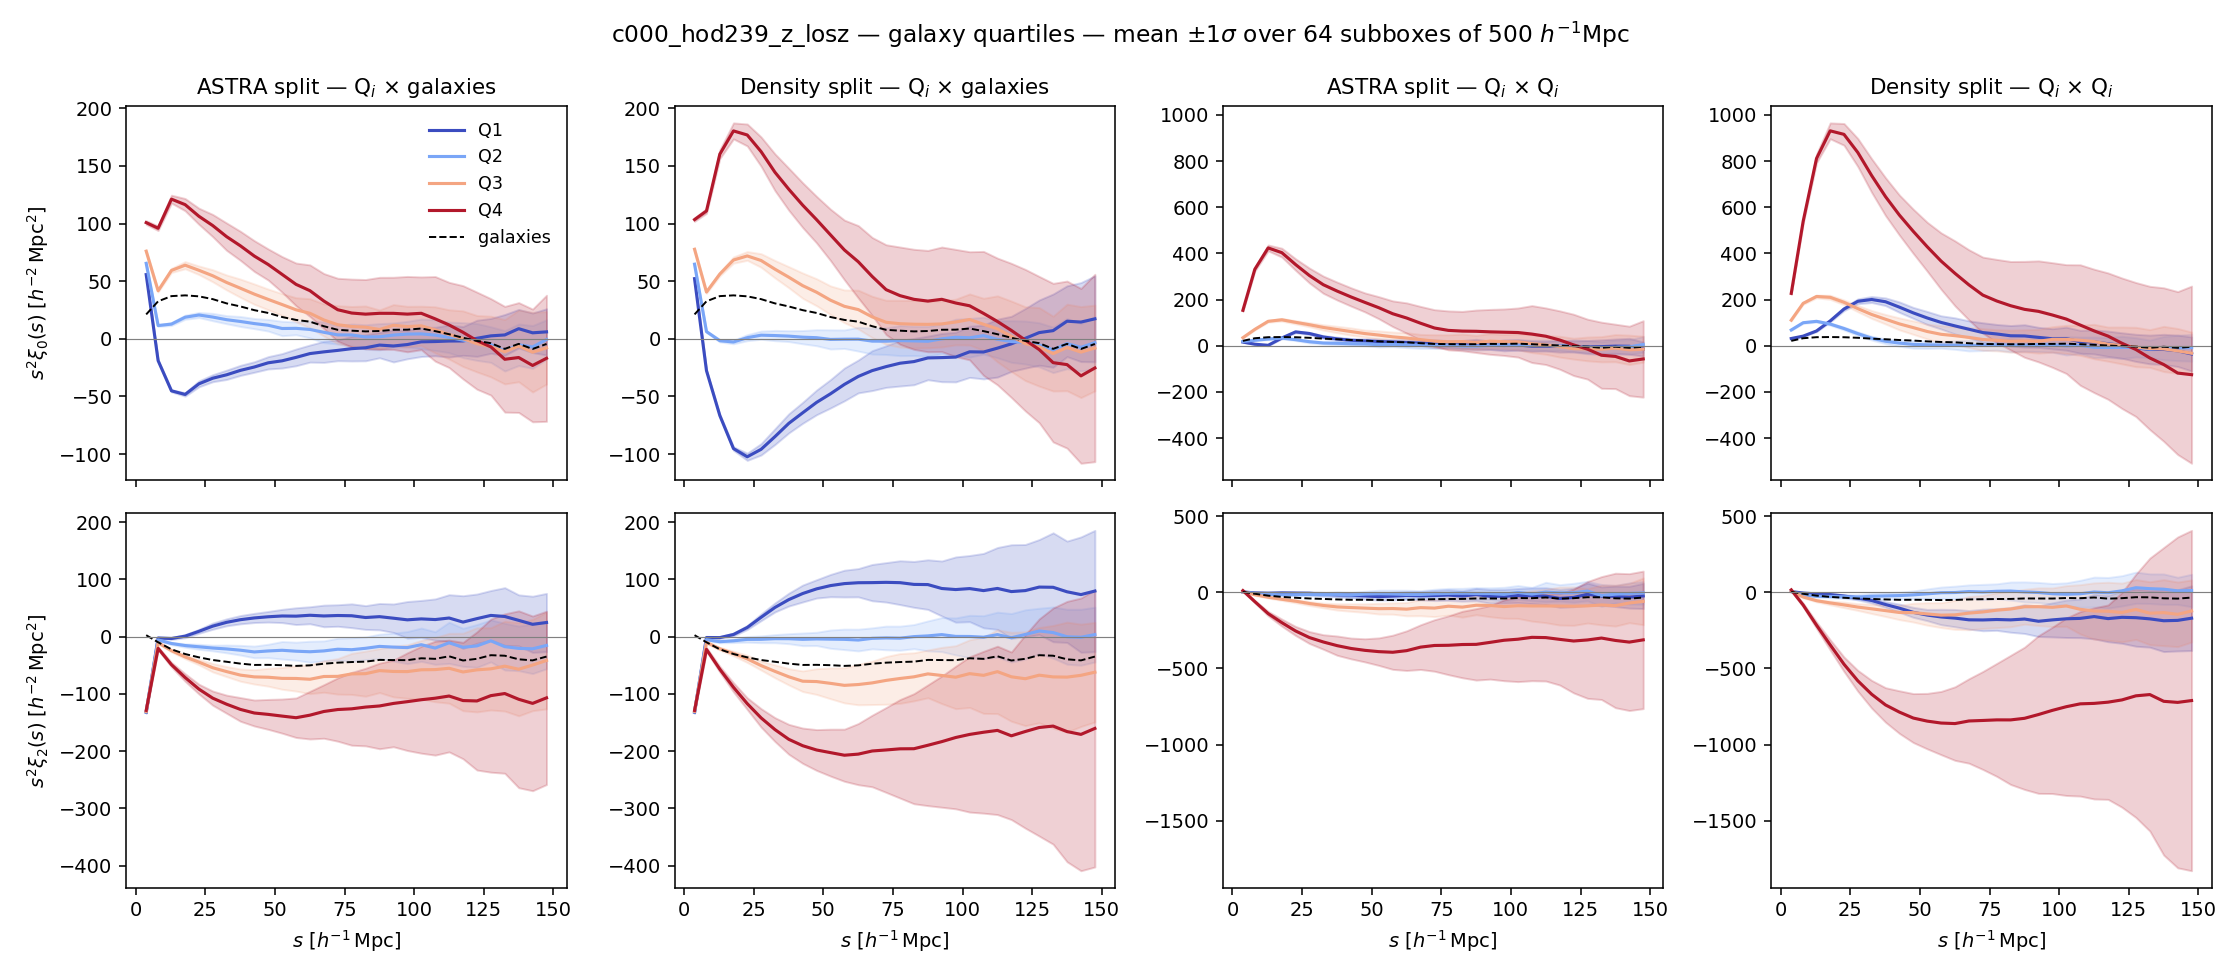
\includegraphics[width=\textwidth]{v2_multipoles_gal.png}
\caption{Same as Figure~\ref{fig:multipoles_rand} for the galaxy quartiles.}
\label{fig:multipoles_gal}
\end{figure*}

\todo{Real-space (r-split) measurements and comparison with redshift space (Fig.~3 of the previous version), once the real-space runs are done.}

% =====================================================================
\section{Covariance, derivatives and Fisher forecasts}
\label{sec:fisher}
% =====================================================================

\subsection{Covariance}

The covariance of each data vector is estimated from the fiducial catalogue (\texttt{c000}, \texttt{hod239}, the c000 draw closest to the centre of the HOD prior), using the 64 subvolumes measured along the three lines of sight: $N_s=192$ samples. The three lines of sight are not independent, so this is an approximation commonly used in simulation-based analyses. The inverse covariance is corrected by the Hartlap factor \cite{Hartlap2007}
\begin{equation}
\hat C^{-1} = \frac{N_s - N_d - 2}{N_s - 1}\, C^{-1},
\end{equation}
where $N_d$ is the size of the data vector. To keep this factor reasonable we restrict the data vectors to $\ell=0,2$, $20 \le s \le 150\Mpch$ in bins of $10\Mpch$ (13 bins per multipole) and, by default, to the cross-correlations of the extreme quartiles Q1 and Q4 ($N_d = 52$ per method, 78 with the 2PCF; Hartlap factors 0.72 and 0.59).

\subsection{Derivatives from HOD-matched pairs}

For each parameter we select one HOD file in each of the two cosmologies of the pair, minimising the distance between the two HOD parameter vectors (normalised to the prior range) plus their distances to the fiducial HOD (Table~\ref{tab:hods}). The selected pairs are about twice closer than random pairs, but a residual mismatch remains (up to $0.3$--$0.4$ of the prior range in single parameters), which we discuss in Section~\ref{sec:discussion}.

The derivative is computed subvolume by subvolume and line of sight by line of sight,
\begin{equation}
\frac{\partial \xi}{\partial\theta} = \frac{1}{N_s}\sum_{k=1}^{N_s} \frac{\xi_k(\theta_+) - \xi_k(\theta_-)}{\theta_+-\theta_-},
\end{equation}
before averaging. Since the two simulations share the same initial conditions and the same random points, cosmic variance and random noise largely cancel in each difference. The error on the mean derivative is estimated from the scatter of the $N_s$ differences.

\begin{table}[h]
\centering\small
\begin{tabular}{lccc}
\toprule
Parameter & HOD files & $|\Delta h|$ & random pairs \\
\midrule
fiducial & c000\_hod239 & -- & -- \\
$\omega_b$ & c100\_hod448 / c101\_hod694 & 0.63 & 1.38 \\
$\omega_{\rm cdm}$ & c102\_hod589 / c103\_hod841 & 0.58 & 1.38 \\
$n_s$ & c104\_hod308 / c105\_hod735 & 0.65 & 1.37 \\
$\sigma_8$ & c112\_hod230 / c113\_hod204 & 0.65 & 1.39 \\
\bottomrule
\end{tabular}
\caption{HOD catalogues used for the covariance and the derivatives. $|\Delta h|$ is the Euclidean distance between the two HOD parameter vectors normalised to the prior range (12 parameters); the last column gives the median for random pairs.}
\label{tab:hods}
\end{table}

\todo{Figure of the derivatives (ASTRA vs DS, random quartiles, $\ell=0,2$) for the four parameters, \texttt{scripts/derivatives.py}.}

\subsection{Fisher matrix}

The Fisher matrix of a data vector $\boldsymbol d$ is
\begin{equation}
F_{ij} = \frac{\partial \boldsymbol d^T}{\partial\theta_i}\, \hat C^{-1}\, \frac{\partial \boldsymbol d}{\partial\theta_j} - \mathrm{Tr}\!\left[\hat C^{-1}\Sigma_{ij}\right],
\end{equation}
where the second term removes the positive bias due to the noise of the estimated derivatives, $\Sigma_{ij}$ being the covariance between the mean derivatives with respect to $\theta_i$ and $\theta_j$. The marginalised errors are $\sigma(\theta_i) = \sqrt{(F^{-1})_{ii}}$. We quote them for the volume of one subvolume, $0.125\,(h^{-1}{\rm Gpc})^3$.

These forecasts are at fixed HOD parameters. They measure the information content of each statistic on the cosmological parameters, not the constraints of a full analysis, in which the HOD parameters are marginalised over.

\subsection{Results}

\todo{Table of marginalised errors for: 2PCF, ASTRA rand, DS rand, ASTRA gal, DS gal, 2PCF+ASTRA, 2PCF+DS (\texttt{scripts/fisher.py}). Triangle plots ASTRA vs DS vs 2PCF and bar chart of $\sigma_{\rm 2PCF}/\sigma$. Scale cut study ($s_{\min}$ = 10, 20, 40, 60). Effect of adding the quartile autos.}

% =====================================================================
\section{Robustness tests}
\label{sec:robustness}
% =====================================================================

\todo{Results of \texttt{scripts/robustness.py}: (i) padding $30\to60\Mpch$, (ii) $N_r/N_g = 1\to2$, (iii) thinning by 2 and 5 (shift of the quartile multipoles in units of the one-subvolume error), (iv) stability of $r$ of the same galaxies under thinning by 2, 5, 10 (Spearman correlation, quartile retention).}

% =====================================================================
\section{Discussion and limitations}
\label{sec:discussion}
% =====================================================================

\paragraph{HOD mismatch in the derivatives.} The emulator catalogues are not HOD-matched across cosmologies. Our selection reduces the mismatch by a factor of two but does not cancel it, so the finite differences contain a residual response to the HOD parameters, smooth in scale and mostly affecting the amplitude. It is expected to matter most for $\sigma_8$, whose effect is also mainly an amplitude. A clean solution is an emulator of the statistics as a function of cosmological \emph{and} HOD parameters, trained on the full Latin hypercube, whose derivatives can be taken at fixed HOD.

\paragraph{Single phase.} All the cosmologies share one set of initial conditions, so the covariance relies on subvolumes of one box, measured along three correlated lines of sight. Larger sets of independent small boxes would remove both the subvolume approximation and the limit on the size of the data vector imposed by the Hartlap factor.

\paragraph{Towards inference.} The natural next step is a simulation-based inference in the spirit of \cite{CuestaLazaro2024}: a neural-network emulator of the ASTRA-split multipoles trained on the 85 cosmologies $\times$ HOD draws, combined with the covariance of this work in an MCMC exploration of the joint cosmological and HOD parameter space.

% =====================================================================
\section{Conclusions}
% =====================================================================

\todo{Conclusions once the Fisher forecasts and robustness tests are final.}

% =====================================================================
\appendix
\section{Reproducibility}
\label{app:repro}
% =====================================================================

All the measurements and figures of this paper are produced by the code at \todo{GitHub URL}, run on the NERSC Perlmutter CPU nodes with the \texttt{cosmodesi} environment:
\begin{lstlisting}[language=bash]
source /global/common/software/desi/users/adematti/cosmodesi_environment.sh main
python scripts/select_hods.py          # Table 2
sbatch slurm/run_catalog.sbatch 0 239 z --los z
python scripts/plot_multipoles.py data/c000_hod239_z_losz.npz
python scripts/derivatives.py
python scripts/fisher.py
python scripts/robustness.py
\end{lstlisting}
Measuring one catalogue (64 subvolumes, ASTRA and density split, 33 statistics) takes $\simeq 8$ minutes on one 128-core node. The HOD catalogues are read from \texttt{/pscratch/sd/n/ntbfin/emulator/hods/z0.5/yuan23\_prior/}.

\begin{table}[h]
\centering\small
\begin{tabular}{lc}
\toprule
Setting & Value \\
\midrule
Subvolumes & $4^3$ of $500\Mpch$ \\
ASTRA padding & $30\Mpch$ (periodic) \\
ASTRA randoms & $N_r = N_g$ \\
DS smoothing & Gaussian, $R_s = 10\Mpch$ \\
DS mesh & $5\Mpch$, CIC \\
Quartiles & 4, equal counts \\
Geometry randoms & $5\,N_g$ per subvolume \\
$s$ bins & $[0,150]\Mpch$, $\Delta s = 5\Mpch$ \\
$\mu$ bins & 120 in $[-1,1]$ \\
Multipoles & $\ell = 0, 2, 4$ \\
Seed & 42 \\
\bottomrule
\end{tabular}
\caption{Numerical settings of the measurements.}
\label{tab:config}
\end{table}

\section{Differences with a first version of the pipeline}
\label{app:v1}

A first version of this analysis averaged the statistics of 64 different HOD files per cosmology to build ``covariance'' and ``derivative'' sets, and measured them in the central $500\Mpch$ cube of each box. We document here why it was abandoned, as these pitfalls are generic to emulator suites:
\begin{enumerate}
\item the HOD files are different HOD models, not realisations: their scatter ($\sim55\%$) dominated the cosmological differences ($\sim1\%$), and the finite differences were compatible with noise (median $|S/N|<1$ per bin for $\omega_b$, $n_s$, $\sigma_8$);
\item pair counts assumed periodic boundary conditions in a non-periodic cut box;
\item the 2PCF used the mid-point line of sight from the centre of the box instead of the axis along which the RSD were applied, which erased the quadrupole;
\item quartiles were computed jointly on galaxies and randoms, giving unequal and realisation-dependent quartile sizes;
\item the Delaunay triangulation was computed on the cut box without periodic padding;
\item ASTRA was first applied to the random catalogue alone (randoms against other randoms), so that the random quartiles carried no information on the galaxy field and their correlations were consistent with zero.
\end{enumerate}

\begin{thebibliography}{99}
\bibitem{Paillas2023} E.~Paillas et al., \emph{Constraining $\nu\Lambda$CDM with density-split clustering}, MNRAS 522, 606 (2023), arXiv:2209.04310.
\bibitem{Paillas2024} E.~Paillas et al., \emph{Cosmological constraints from density-split clustering in the BOSS CMASS galaxy sample}, arXiv:2309.16541 (2024).
\bibitem{CuestaLazaro2024} C.~Cuesta-Lazaro et al., \emph{SUNBIRD: a simulation-based model for full-shape density-split clustering}, MNRAS (2024), arXiv:2309.16539.
\bibitem{ASTRA} \todo{ASTRA reference (Forero-Romero et al.).}
\bibitem{Maksimova2021} N.~A.~Maksimova et al., \emph{AbacusSummit: a massive set of high-accuracy, high-resolution N-body simulations}, MNRAS 508, 4017 (2021), arXiv:2110.11398.
\bibitem{Yuan2022} S.~Yuan et al., \emph{AbacusHOD: a highly efficient extended multitracer HOD framework}, MNRAS 510, 3301 (2022), arXiv:2110.11412.
\bibitem{Yuan2023} \todo{Reference of the yuan23 HOD prior used for the DESI emulator catalogues.}
\bibitem{LandySzalay1993} S.~D.~Landy \& A.~S.~Szalay, ApJ 412, 64 (1993).
\bibitem{Sinha2020} M.~Sinha \& L.~H.~Garrison, \emph{Corrfunc}, MNRAS 491, 3022 (2020).
\bibitem{Hartlap2007} J.~Hartlap, P.~Simon \& P.~Schneider, A\&A 464, 399 (2007).
\end{thebibliography}

\end{document}
